\documentclass{article}
\usepackage[left=2cm,right=2cm,top=2cm,bottom=2cm]{geometry} 
\usepackage{graphicx} 
\usepackage[spanish]{babel}
\usepackage{titlesec}
\setcounter{secnumdepth}{3}

%--------------------- Custom commands ------------------------------
\newcommand*\rbreak{\par\noindent\linebreak}
\newcommand*\casoheadera[2]{
	\textbf{#1} & 
	\parbox[t]{12cm}{#2} \\\hline
}
\newcommand\casoheaderb[2]{
	\multicolumn{2}{|l|}{
		\parbox[t]{15cm}{ \textbf{#1} \\ #2 \\ } 	
	} \\\hline
}
%------------------------ Constants ---------------------------------
\newcommand{\nombre}{Renato Josué Flores Pérez}
\newcommand{\carnet}{201709244}
\newcommand{\titulo}{Rescantando a MasterDevelop}
\graphicspath{{/home/renato/latex/general/master-develop/images/}}

%------------------------ Title formating --------------------------

\author{\nombre , \carnet}
\title{\textbf{\Huge\titulo}}

%------------------------- Document --------------------------------
\begin{document}
\maketitle
\section{¿Qué opinas sobre la decisión de Armando Guerra de no invertir más recursos humanos
    y económicos en un producto de software innovador?}
\begin{itemize}
	\item  La descisión de Armando de recortar el personal para
		ahorrar recursos y disminuir el presupuesto
		es sin duda la solución más sencilla para resolver
		los déficits terribles en que se encuentra la empresa.

	\item La solución de Armando es únicamente una solución
		a corto plazo y de hecho, 
		estoy convencido de que a largo plazo,
		Softics disminuirá su presencia en el mercado, 
		perderá relaciones importantes con sus clientes e
		inclusive podría llegar a la quiebra de seguir un 
		rumbo similar.

	\item Debe encontrarse un equilibrio entre el Ahorro
		y la Inversión en investigación, desarrollo e 
		innovación. Esto no puede ser pasado por alto,
		más aún en una empresa como Softics, cuyo lema
		principal es la innovación y desarrollo de 
		sistemas de información. De lo contrario, 
		Softics se estancará y no será capaz de 
		seguir adelante, perdiendo toda ventaja contra sus
		competidores y eventualmente cayendo en la obsolencia.
\end{itemize}

\section{¿Qué conocimientos, habilidades y actitudes debe tener Luis para sortear con éxito
    las dificultades que enfrenta al elaborar la propuesta de rescate de MasterDevelop?}
    \subsection{Conocimientos}
    \subsubsection{Definición de valor para el cliente}
    	Es fundamental que Luis posea una clara definición de lo que
	significa valor para cada uno de sus clientes, tanto actuales
	como potenciales. Esto es de vital importancia para poder 
	identificar éxitosamente que funcionalidades y tareas 
	deben ser priorizadas para su implementación y que 
	funcionalidades puden ser retrasadas o incluso deprecadas
	y removidas del proyecto si no aportan valor al cliente.
    \subsubsection{Noción de calidad}
    	Una vez Luis conozca la definición de valor según el cliente,
	debe tener una firme noción de calidad y de cómo se espera 
	confirmar y probar dicha calidad, para poder asegurar
	que las funcionalidades del sistema que espera utilizar el 
	cliente, efectivamente funcionen correctamente y produzcan 
	los resultados esperados.
    \subsubsection{Entendimiento del organigrama de la empresa}
    	Es fundamental que Luis conozca a fondo el organigrama 
	vigente de la empresa, para de esta forma poder elaborar un 
	plan de comunicación efectivo que facilite el intercambio
	de información pertinente al proyecto dentro de la empresa.
    \subsubsection{Conocer los casos de uso prácticos de sus clientes}
    	Es importante que Luis posea un conocimiento claro de los
	casos de uso prácticos que sus clientes le dan al 
	MasterDevelop, para de esta forma poder estudiar de que forma
	se pueden mejorar, extender y otorgar valor agregado a sus
	clientes.
    \subsubsection{Entender la importancia de pruebas automatizadas}
    	Para poder probar la calidad del Software es necesario que
	Luis posea conocimiento de la importancia de pruebas 
	automatizadas y de esta forma implementarlas él mismo o 
	contratar a un ingeniero de cálidad que las implemente por él.
	Siempre en base a los criterios de calidad definidos para
	MasterDevelop que Luis sobre los cuáles Luis debe
	tener pleno conocimiento.
    \subsubsection{Una forma de modelado estándar para expresar
    sus ideas y conceptos a su equipo de desarrollo}
    	Es de vital importancia que Luis sea altamente versado en 
	algún lenguaje de modelado estándar que le permita
	expresar sus ideas y diseños a su equipo de desarrollo.
	Se recomienda UML por ser el lenguaje por excelencia de 
	modelado de Sistemas. Por tanto, Luis debe ser altamente
	versado en UML al igual que su equipo, para poder comunicar
	ideas y diseños del sistema de manera entendible, rápida
	y eficaz.
    \subsubsection{Estadística e Inferencia}
    	Sería muy útil, más no obligatorio, que Luis posea 
	conocimientos intermedio-avanzados sobre temas de Estadística
	e Inferencia, para de esta forma poder llevar a cabo análisis
	de tendencias de uso, históricos de gastos, entre otros 
	que le serían útiles para descubrir funcionalidades 
	desperdiciadas por los usuarios o puntos críticos de gran 
	acumulación de costos y tiempo en el proyecto.

    \subsection{Actitudes}
    \subsubsection{Hacer las cosas, no solo pensarlas}
    Para rescatar a MasterDevelop, es de vital importancia
    que Luis posea una actitud proactiva y se encargue de llevar
    a cabo sus planes, no solamente pensarlos. Debe estar dispuesto
    a tomar medidas y realizar las tareas que otros no se atreverían 
    o no podrían hacer.
    \subsubsection{Saber cómo priorizar}
    Luis debe tener una actitud que sepa respetar prioridades
    y debe saber como priorizar tareas según su nivel de importancia
    y urgencia.
    \subsubsection{Disposición de aprendizaje continuo}
    Para rescatar a MasterDevelop y continuar innovando, es de vital
    importancia que Luis adopte una actitud de aprendizaje continuo
    y nunca piense que lo sabe todo o que no se puede mejorar.
    \subsubsection{No hacer excusas}
    Si algo falla durante la ejecución de su plan de rescate, es 
    importante que Luis adopte una actitud que le permita asumir
    responsablemente las consecuencias de dichos fallos, en vez
    de culpar a otros o hacer excusas. 
    \subsubsection{No darse por vencido}
    No darse por vencido, Luis ya ha demostrado tener esta actitud
    y es efectimante importante para poder llevar a cabo el plan
    de rescate de MasterDevelop. Siempre y cuando no se haya tocado
    fondo, siempre hay una salida y debe trabajarse arduamente para
    llegar a ella. Luis a demostrado claramente esta actitud.
    \subsubsection{Atención al detalle}
    No hay tarea lo suficientemente pequeña como para ser
    sobreestimada. Si una tarea está planeada para su ejecución debe
    ser realizada correctamente, prestando especial atención a los
    detalles. Nunca se debe suponer ni sobreestimar nada.

    \subsection{Habilidades}
    \subsubsection{Liderazgo}
    Como es de esperarse, la habilidad principal que Luis debe
    poseer para llevar a cabo éxitosamente el rescate de MasterDevelop
    es la de liderazgo, Luis será responsable no solamente de 
    planear el rescate y delegar las tareas. Luis debe hacerse 
    cargo por velar por que dichas tareas se cumplan, tomar medidas,
    incentivar al equipo, definir los goles del proyecto y guiar
    a su equipo hacia tales goles.
    \subsubsection{Comunicación}
    Para todo jefe de proyectos es indispensable su habilidad para la
    comunicación, Luis debe ser capaz de expresar sus ideas, diseños,
    preocupaciones y sugerencias efectivamente tanto a sus superiores
    como a sus delegados.
    \subsubsection{Planificación}
    Sin duda es importante que Luis posea una alta habilidad para
    la planeación de tareas y que tome en cuenta el perfil de los
    miembros de su equipo, los recursos financieros disponibles,
    el tiempo estipulado y los recursos digitales a su 
    disposición.
    \subsubsection{Manejo del riesgo}
    En todo proyecto siempre hay riesgos, y los hay más aún en un 
    proyecto de rescate. Luis debe ser habilidoso en la forma
    en que se prepara y reacciona a los posibles riesgos que puedan
    presentarse durante el rescate de MasterDevelop. Luis siempre
    debe estar preparado.
    \subsubsection{Negociación}
    Finalmente, pero no menos importante, Luis debe ser capaz 
    de llevar a cabo negociaciones importantes con sus superiores
    para acordar y llegar a un convenio respecto a los recursos
    necesarios que serán dispuestos para llevar a cabo el 
    rescate de MasterDevelop. 

\section{¿Consideras que Luis Aguilar era o no una persona idónea para elaborar con éxito un 
    plan de rescate para MasterDevelop?}

	Si. Considero que Luis Aguilar es, efectivamente la persona
	idónea para elaborar y llevar a cabo el plan de rescate
	de MasterDevelop. Luis posee una alta trayectoria (más de
	quince años) en el área de innovación, por lo que una
	de sus principales características es su alta habilidad de
	adaptación y fácilidad de adoptar los cambios. Esto sin duda
	le permitirá adaptarse al nuevo modelo de negocios de 
	Softics y poder sortear con éxito el drástico recorte de 
	presupuesto que estaba su disposición en el pasado.
	\\\\
	Además de su habilidad para adaptarse al cambio, Luis
	estuvo presente en todo momento durante el desarrollo de
	MasterDevelop, desde su concepción como una idea, hasta
	su implementación en su primera versión y posteriores que
	situaron a MasterDevelop 3.0 como uno de los productos
	insignia de Softics. Esta experiencia sin duda es 
	indispensable para que Luis pueda evaluar que características
	del software mejorar, que características remover y que 
	se puede agregar para rescatar la viabilidad de 
	MasterDevelop como un producto competitivo en el mercado.
	\\\\
	Además de su experiencia en el desarrllo del sistema y 
	de su experiencia en el área académica, otra habilidad
	importantísima que indudablemente califica a Luis para
	tomar la responsabilidad de enunciar y llevar a cabo el 
	plan de rescate de MasterDevelop, es su conocimiento y 
	relaciones actuales con los clientes de Softics que ya han 
	adoptado a MasterDevelop como parte de sus herramientas. 
	Al estar Luis familiarizado con ellos, este podrá identificar
	de mejor manera que exactamente esperan los clientes obtener
	de MasterDevelop y de como poder mantener el producto de
	manera que sea posible su rentabilidad e innovación.

\section{¿Qué tipo de productos y servicios podrían 
integrarse a MasterDevelop para ser económicamente 
auto-sustentable dadas las restricciones que lo limitaban?}

\subsection{Diagramas de casos de uso}
\begin{figure}[ht]
	\centering
        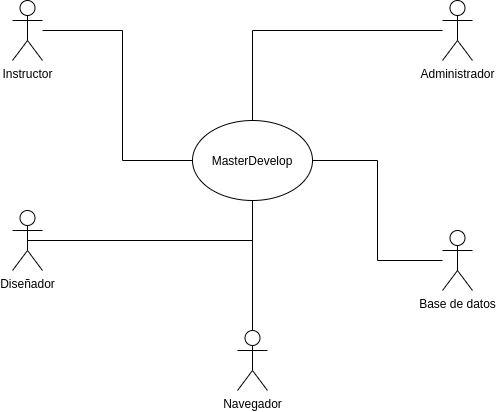
\includegraphics[width=400px,keepaspectratio]{casos-uso-alto-nivel.png}
                 \caption{Diagrama de casos de uso de más alto nivel}
\end{figure}	
\clearpage
\begin{figure}[ht]
        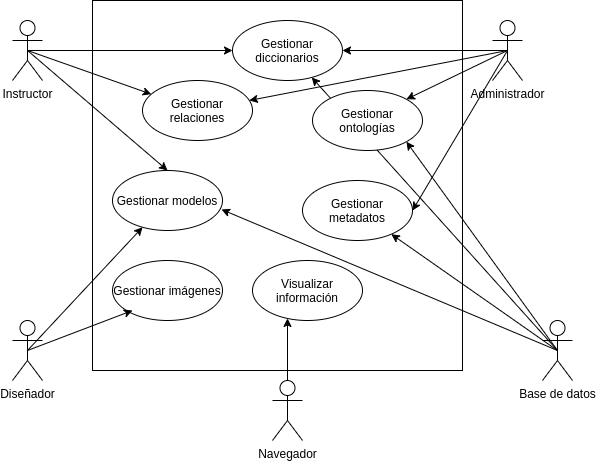
\includegraphics[width=\textwidth,keepaspectratio]{casos-uso-general.png}
                 \caption{Diagrama de casos de uso de alto nivel}
\end{figure}	

\clearpage

\begin{figure}[ht]
	\centering
        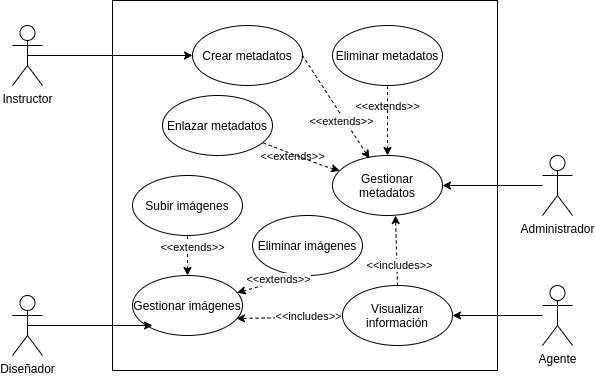
\includegraphics[width=400px,keepaspectratio]{extended-1.png}
                 \caption{Diagrama de casos de uso expandido}
\end{figure}	

\begin{figure}[ht]
	\centering
        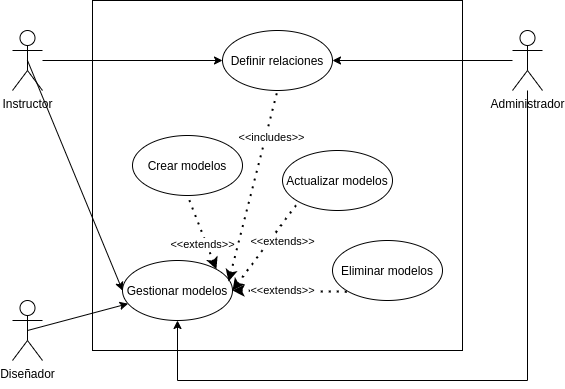
\includegraphics[width=400px,keepaspectratio]{extended-2.png}
                 \caption{Diagrama de casos de uso expandido}
\end{figure}	

\subsection{Casos de uso}
\subsubsection{Crear diccionarios}
\begin{tabular}{  | m{3cm} | m{12cm} | }
	\hline
	\casoheadera{Nombre}{Crear diccionarios}
	\casoheadera{Autor}{\nombre}
	\casoheadera{Fecha}{\today}
	\casoheaderb{Descripción}{
		Los diccionarios ayudan a la web semántica a dar significado 
		a las palabras encontradas en los textos de las vistas que 
		desean crear los usuarios. Ayudan a identificar sustantivos, verbos,
		artículos, adverbios y demás en base al contexto, la semántica y los
		metadatos del documento. Crear y definir diccionarios es de vital
		importancia para la web semántica por esta razón.

	}
	\casoheaderb{Actores}{
		Administrador, Instructor
	}
	\casoheaderb{Precondiciones}{
		Haber creado uno o más modelos.
	}
	\casoheaderb{Flujo Normal}{
		\begin{enumerate}
			\item Ingresar al panel de administración de MasterDevelop.
			\item En la barra de navegación, seleccionar Diccionarios.
			\item En el menú que se presenta, seleccionar crear Diccionario.
			\item Llenar el diccionario a mano (no recomendable) o seleccionar 
				importar. MasterDevelop soporta diccionarios simples en 
				formato XML, RDF, TOML, JSON y YAML.
		\end{enumerate}
	}
	\casoheaderb{Poscondiciones}{
		\\
		El diccionario será registrado y estará disponible para su posterior
		uso por parte del mecanismo de inferencias y la asignación automática 
		de metadatos.
	}
\end{tabular} 
% ''''''''''''''''''''''''''''''''''''''''''''''''''''''''''''''''''''''''''''''''''''
\subsubsection{Editar diccionarios}
\begin{tabular}{  | m{3cm} | m{12cm} | }
	\hline
	\casoheadera{Nombre}{Editar diccionarios}
	\casoheadera{Autor}{\nombre}
	\casoheadera{Fecha}{\today}
	\casoheaderb{Descripción}{
		Si bien es sencillo importar diccionarios, estos comúnmente
		son conjuntos simples de clave valor. Sin embargo, un 
		diccionario mucho más útil es aquel que aporta anotaciones,
		tipos, temas, sinónimos y relaciones entre las palabras. MasterDevelop
		soporta la asignación y aplicación de estas propiedades. Este
		caso de uso demuestra como pueden agregarse estas propiedades
		para enriquecer los diccionarios creados previamente de Master
		Develop
	}
	\casoheaderb{Actores}{
		Administrador, Instructor
	}
	\casoheaderb{Precondiciones}{
		Haber creado uno o más diccionarios.
	}
	\casoheaderb{Flujo Normal}{
		\begin{enumerate}
			\item Ingresar al panel de administración de MasterDevelop.
			\item En la barra de navegación, seleccionar Diccionarios.
			\item En el menú que se presenta, seleccionar editar Diccionario.
			\item En el drop down de diccionarios registrados, seleccionar
				el diccionario de interés.
			\item Utilizar la barra de búsqueda y los filtros para navegar
				con facilidad el diccionario. Por cada término de interés,
				seleccionar editar.
			\item Editar los datos del término seleccionado o agregar 
				la información pertinente.
		\end{enumerate}
	}
	\casoheaderb{Poscondiciones}{
		\\
		El diccionario será enriquecido con la información extra disponible 
		a cada término y como concecuencia, las inferencias y la asignación
		de metadatos será más acertada y rápida.
		}
\end{tabular} 
% ---------------------------------------------------------------------------------
\subsubsection{Definir relaciones}
\begin{tabular}{  | m{3cm} | m{12cm} | }
	\hline
	\casoheadera{Nombre}{Definir relaciones}
	\casoheadera{Autor}{\nombre}
	\casoheadera{Fecha}{\today}
	\casoheaderb{Descripción}{
		Una de las funciones más útiles de MasterDevelop
		y que sin duda es un factor decisivo al momento de
		posicionarlo como un producto innovador y útil, es la
		habilidad de poder definir relaciones entre vistas, 
		modelos y ontologías. De esta forma, la generación de 
		inferencias y sugerencias útiles para el usuario se vuelve
		una realidad. Ya que de lo contrario, el tiempo de búsqueda que 
		le llevaría al sistema para análizar todos los diccionarios, 
		ontologías y modelos para calcular sus inferencias sería demasiado
		prologado debido a su gran volumen y en consecuencia el usuario
		marcaría la prolongada espera como tediosa y MasterDevelop como
		poco útil y práctico.
	}
	\casoheaderb{Actores}{
		Administrador
	}
	\casoheaderb{Precondiciones}{
		\begin{enumerate}
			\item Estar registrado en el sistema como usuario administrador
			\item Haber definido una o más ontologías
			\item Haber definido uno o más diccionarios
			\item Haber definido uno o más modelos
			\item Haber definido una o más vistas
		\end{enumerate}
	}
	\casoheaderb{Flujo Normal}{
		\begin{enumerate}
			\item Ingresar a la página de administración de MasterDevelop.
			\item Seleccionar la opción de relaciones.
			\item El sistema mostrará un mapa conceptual gráfico que le ayudará
				al administrador a comprender las relaciones actualmente
				definidas en el proyecto.
			\item El usuario será capaz de crear, eliminar o modificar relaciones
				según le convenga con ayuda de una interfaz gráfica.
		\end{enumerate}
	}
	\casoheaderb{Poscondiciones}{
		\\
		La red de relaciones del sistema que puede crear el usuario a partir
		de esta herramienta le será de vital utilidad al sistema mientras este
		crece en robustez y dominio de datos. La red de relaciones le permitirá
		al sistema de inferencias saber donde priorizar sus búsquedas y le permitirá
		obtener resultados válidos con una gran velocidad.
	}
\end{tabular} 
%--------------------------------------------------------------------------------------
\subsubsection{Crear ontologías}
\begin{tabular}{  | m{3cm} | m{12cm} | }
	\hline
	\casoheadera{Nombre}{Crear Ontologías}
	\casoheadera{Autor}{\nombre}
	\casoheadera{Fecha}{\today}
	\casoheaderb{Descripción}{
		Si bien el Diccionario representa un conjunto de datos
		que poseen nombre, significado y tipo. Este es de poca 
		utilidad si no está bien definido qué es cada tipo y que 
		tipos se encuentran disponibles. Los tipos por defecto son 
		aquellos encontrados en el lenguaje natural que los desarrolladores
		de MasterDevelop consideraron oportunos para su implementación.
		Algunos ejemplos son ``Adverbios'', ``Artículos'', ``Pronombres'',
		``Sustantivos'', ``Verbos''. Sin embargo, estos tipos pueden ser
		extendidos o removidos por el usuario. Nuevos tipos pueden ser definidos
		y cargados al sistema. Al conjunto de tipos junto a su definición y
		propiedades MasterDevelop le llama Ontología. 
	}
	\casoheaderb{Actores}{
		Administrador, Instructor.
	}
	\casoheaderb{Precondiciones}{
		\begin{enumerate}
			\item Estar registrado en el sistema como usuario administrador.
		\end{enumerate}
	}
	\casoheaderb{Flujo Normal}{
		\begin{enumerate}
			\item Ingresar a la página de administración
			\item Seleccionar la opción Ontologías.
			\item Seleccionar la opción Crear.
			\item Seleccionar la opción Agregar Tipo.
			\item Llenar la información requerida por el Sistema
				para la definición de un Tipo.
		\end{enumerate}
	}
	\casoheaderb{Flujo Alternativo}{
		\\
		El sistema también soporta la carga de nuevos Tipos 
		de manera masiva. Estos deben ser cargados en un documento
		con formato XML que defina de manera concisa e inequivoca a cada
		tipo que será parte de la Ontología. Si alguno de los tipos
		a cargar viola las reglas de integridad de Tipos definidas
		por el sistema se alertará al usuario y se rechazará el archivo
		entero.
	}
	\casoheaderb{Poscondiciones}{
		\\
		El usuario será capaz de consultar, manipular y eliminar la Ontología
		creada. La ontología quedará registrada en el sistema para su posterior
		uso al momento de relacionarla con el resto de elementos del sistema.
	}
\end{tabular} 

\subsubsection{Asignar Metadatos}
\begin{tabular}{  | m{3cm} | m{12cm} | }
	\hline
	\casoheadera{Nombre}{Asignar Metadatos}
	\casoheadera{Autor}{\nombre}
	\casoheadera{Fecha}{\today}
	\casoheaderb{Descripción}{
		Los metadatos en el contexto de MasterDevelop son 
		pequeñas piezas de información que se le añaden 
		a un documento o vista que le permite a la red semántica
		identificar su nombre, tamaño, categoría, tema y demás 
		información relevante para que el sistema de inferencias
		sea capaz de relacionar el documento con los modelos,
		diccionarios u ontologías definidas en el sistema. Los
		metadatos pueden ser añadidos a un documento o vista de
		forma manual o automática. Esta última es una de las
		funcionalidades que hacen a MasterDevelop tan útil
		y reconocido.
	}
	\casoheaderb{Actores}{
		Diseñador, administrador, Instructor
	}
	\casoheaderb{Precondiciones}{
		\begin{enumerate}
			\item Estar registrado en el sistema.
			\item Haber creado una o más vistas.
		\end{enumerate}
	}
	\casoheaderb{Flujo Normal}{
		\begin{enumerate}
			\item Ingresar a la página de inicio del sistema.
			\item Seleccionar la opción Gestionar Vistas.
			\item Escoger la vista a la cuál se le desea asignar metadatos.
			\item Seleccionar la opción Asignar Metadato.
			\item Llenar el formulario que se le presentará con la información
				relevante para definir el metadato.
			\item Seleccionar guardar.
		\end{enumerate}
	}
	\casoheaderb{Flujo Alternativo}{
		La forma en que se asignan metadatos de manera automática 
		es bastante simple. El usuario simplemente debe enlazar la
		vista objetivo con un modelo en concreto. El sistema posteriormente
		se encargará de realizar un análisis de inferencia recursivo en busca
		de documentos similares relacionados con dicho modelo y creará 
		metadatos relevantes para el nuevo documento. La certeza de estos metadatos
		dependerá de la cantidad de documentos cargados al sistema y la robustez de 
		las relaciones dentro de la red semántica definidas por el usuario. Por esta razón
		esta opción no es recomendada cuando aún se están creando los primeros documentos
		de MasterDevelop. Sin embargo, es extremadamente útil cuando el
		sistema ha crecido y en este momento facilitará al usuario 
		la creación de nuevas vistas, volviendolo en cierto modo, auto-sustentable
		a partir de este punto.
	}
	\casoheaderb{Poscondiciones}{
		\\
		El usuario será capaz de recibir inferencias y sugerencias cuando visualice
		sus documentos por medio del navegador en base a los metadatos
		asociados a la vista en cuestión.
	}
\end{tabular} 

\subsubsection{Gestión de imágenes}
\begin{tabular}{  | m{3cm} | m{12cm} | }
	\hline
	\casoheadera{Nombre}{Gestión de imágenes}
	\casoheadera{Autor}{\nombre}
	\casoheadera{Fecha}{\today}
	\casoheaderb{Descripción}{
		El manejo de recursos multimedia es sin duda 
		clave para cualquier red web. MasterDevelop 
		por el momento soporta únicamente el manejo de 
		imágenes. Sin embargo, si el proyecto es rescatado 
		éxitosamente, se planea introducir soporte para 
		otros formatos multimedia en la versión 4.0
	}
	\casoheaderb{Actores}{
		Diseñador
	}
	\casoheaderb{Precondiciones}{
		\begin{enumerate}
			\item Haber creado una o más vistas
		\end{enumerate}
	}
	\casoheaderb{Flujo Normal}{
		\begin{enumerate}
			\item Ingresar a la página de inicio del sistema.
			\item Seleccionar Gestionar Vistas.
			\item Seleccionar la Vista a la cuál se le desea adjuntar imágenes.
			\item Seleccionar Editar.
			\item Seleccionar la opción Agregar Imágenes
			\item La interfaz de usuario cambiará a un formato que no le permitirá 
				editar texto, sin embargo creará un formato Drag and Drop sobre el 
				cuál el usuario será capaz de arrastrar y posicionar imágenes
				donde considere pertinente.
			\item Seleccionar Guardar
			\item La vista será actualizada e incorporará las imágenes que ha decidido 
				el usuario.
		\end{enumerate}
	}
	\casoheaderb{Poscondiciones}{
		\\
		El usuario podrá navegar y visualizar las imágenes en el navegador y 
		asímismo será capaz de editarlas o removerlas en caso de ser necesario.
	}
\end{tabular} 
\clearpage

\begin{figure}[ht]
	\centering
        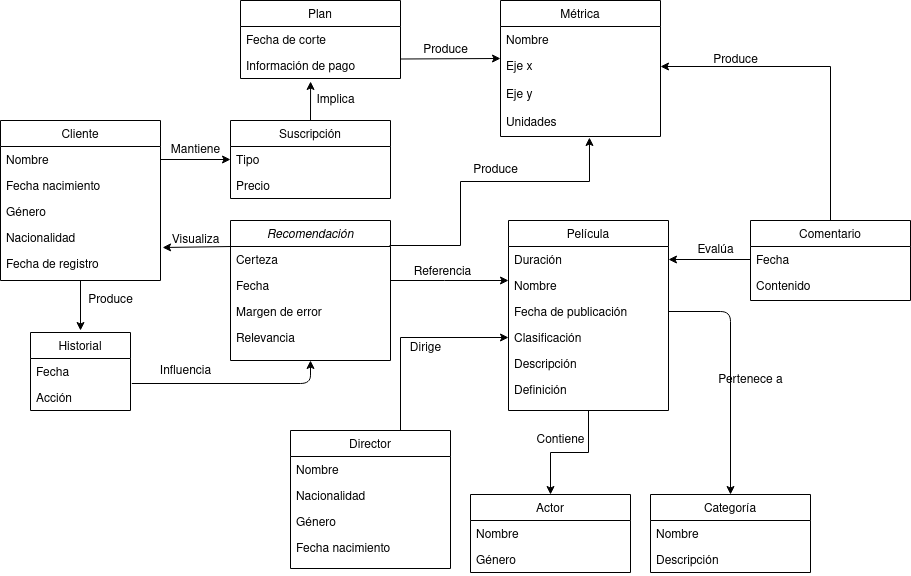
\includegraphics[width=\textwidth,keepaspectratio]{modelo-conceptual.png}
                 \caption{Modelo conceptual, identificando los principales objetos de negocio}
\end{figure}	

\subsection{Resumen}
En resumen, los nuevos productos o servicios que deberían incomporarse, 
luego de haber modelado el negocio, reconocido los actores y haber
realizado el análisis de requerimientos son los siguientes.
\subsubsection{Crear un nuevo navegador}
Actualmente, MasterDevelop crea portales web de manera semi-automatica 
que son desplegables y consumidos sobre navegadores tradicionales. Sin
embargo, el desarrollo de un nuevo navegador, lo cual es mucho más
viable ahora debido a la precencia de éxitosos navegadores de código
abierto como Chromium o Firefox pueden servir de base o inspiración.
Este nuevo navegador tendría la ventaja que no necesitaría de un proceso
de compilación para que el portal creado por el usuario sea útil y 
consumible. Este nuevo navegador también ofrecería la ventaja
que el sistema de inferencias y sugerencias estaría implementado dentro
del navegador, agregando una experiencia mucho más enriquecedora 
e interactiva para el usuario.
\subsubsection{Añadir material didáctico}
Los conceptos de inferencia, sintaxis, ontologías, contexto, significado,
relaciones, búsqueda recursiva, entre otros serán una de las propiedades 
más atratactivas para las entidades académicas al evualuar el producto.
Por lo que la creación de tutoriales, ejemplos y documentación detallada
dentro del propio sistema y fácilmente accesibles para el usuario 
promoverá su nuevo enfoque académico además que disminuirá la necesidad
de personal de soporte técnico para la solución de dudas comúnes.
\subsubsection{Mejorar el sistema de inferencias}
La red semántica en que se basa actualmente MasterDevelop es sin duda
innovador y amigable. Sin embargo, la eficacia de estas inferencias 
puede ser mejorada al introducir conceptos como los metadatos y 
al definir peso para cada relación. La integración de metadatos y 
pesos en las relaciones le añadirá al mecanismo de inferencias la posibilidad
de calcular rutas de búsqueda mucho más eficaces para el recorrido del 
grafo de la red semántica. Permitiendo la implementación de algoritmos de 
recorrido basados en el Algoritmo de Dijkstra.

\section{¿Cómo resolverías el caso de mantener vivo a Master Develop?}
\subsection{Aplicar la filosofía Lean}
Debido a la naturaleza de la problemática que enfrenta Softics, es preciso 
adoptar la filosofía Lean para el desarrollo y mantenimiento del software.
Esto implica que el primer paso debe ser entender y tener bien definido
el significado de valor para cada uno de los clientes. En base a esta
información se debe crear un mapa de procesos que identifiquen todos los
procesos que están involucrados con el sistema. En base a este mapa y 
la definición de valor del cliente, se debe proceder a seleccionar cuidadosamente
los procesos más críticos e importantes, así como los procesos que no aportan 
valor al cliente en lo absoluto y deben ser eliminados.
\\\\
Una vez identificados y eliminados los desperdicios presentes en el
proyecto se obtendrá un recorte de gastos y ahorro considerable.
Lo cual se acopla apropiadamente a las nuevas políticas de
negocio de Softics.
\subsection{Cambiar el modelo de negocio}
Actualmente, Softics utiliza un modelo de licencia de código propietario
para la venta de MasterDevelop así como un plan de soporte técnico
y consultoría. Si bien el plan de soporte técnico representa una gran parte de
las ganacias de Softics en cuanto a MasterDevelop, esta estrategia dejará de 
ser viable en el futuro cercano debido al recorte de personal y en consecuencia
dificultad de proveer soporte técnico para nuevos clientes. Por esta razón,
se sugiere cambiar el modelo de negocio sobre el cuál se basa la venta y 
publicidad de MasterDevelop por un enfoque más académico. Es decir, 
dada la innovación inherente del producto y el alta estima hacia Softics
por parte del estado como empresa tecnológica nacional, deben aprovecharse
estas propiedades y vender una versión del software con un enfóque didáctico
y académico. Los posibles clientes deben ser universidades nacionales e 
institutos de enseñanza técnica. De esta forma, la necesidad de soporte técnico
dedicado podrá ser reducido en gran medida y reemplazado por modelos de subscripción
por parte de entidades educativas que pagarán por el software y clases de capacitación
de personal inicial. Una vez esté capacitado el personal educativo que elija nuestro
producto ellos se encargarán de enseñar su uso a sus propios alumnos y de proveer el 
soporte técnico durante los laboratiorios o actividades que se lleven acabo.
\\\\
Nuevamente, cabe recalcar la ventaja que posee MasterDevelop para ser distribuído como 
material académico, puesto que será una gran oportunidad para distintas organizaciones
educativas poder utilizar material nacional de alta calidad que les permita enseñar conceptos
clave sobre redes, hipertexto, redes semánticas, ontologías digitales, compiladores, 
interpretes, entre otros conceptos clave que se encargan del correcto funcionamiento de
MasterDevelop.
\subsection{Autosostenibilidad}
Una vez adoptado el nuevo modelo de negocio y luego de negociar éxitosamente algunos
acuerdos con diferentes instituciones educativas entonces deberá prestarse especial 
atención a las capacitaciones del personal que impartirá los cursos de interés. 
Este proceso podrá requerir de una inversión de recursos considerable, sin embargo estos
recursos financieros serán cobrados a las instituciones como parte de los costos
de distribución e instalación. 
\\
Una vez las capacitaciones hayan finalizado, el 
proyecto será autosustentable, ya que el personal interno de las insituciones estará
calificado y será responsable de dar el soporte técnico necesario a sus alumnos, 
provocando que Softics se preocupe solamente por cobrar las cuotas de uso mensuales o anuales.

\end{document}
